\chapter{Procedure}

\section{Geometry of the Setup}
\begin{figure}[tbp]
	\centering
	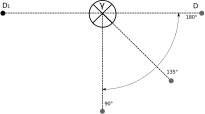
\includegraphics[width=0.5\textwidth]{./img/setup.pdf}
	\caption[Geometry of the Setup]{\textbf{Geometry of the Setup} Detector $D_2$ moves between angles 180, 135 and 90 degrees, while detector $D_1$ is at a fixed position and defines the quantization axis.}
	\label{fig:setup}
\end{figure}
The setup consists of two detectors, discussed in \autoref{sec:detectors}, centered around the $\gamma$-source, as can be seen in \autoref{fig:setup}.
As both detectors are located at a certain distance from the radiation source, the solid angle of detected radiation has to be accounted for in the analysis.
Unfortunately, these corrections are not the same for all measurement series, as the used construction's detector arms vary in distance.

\section{Measurement}
\begin{figure}[tbp]
	\centering
	\includegraphics[width=0.5\textwidth]{./data/plots/e-spectrum.pdf}
	\caption[First energy spectrum]{\textbf{First energy spectrum} Features a back-scatter peak, compton edge and two photo peaks corresponding to the observed decay cascade.}
	\label{fig:e_spectrum}
\end{figure}
To make sure both detector channels have the same energy scale and to determine a threshold, the spectrum of the first measurement is examined.
\autoref{fig:e_spectrum} shows this energy spectrum.
An energy threshold is selected at 7000, isolating the higher energy photopeak.\todo{Actually, I think I was right the first time. Not being able to detect the lower energy photons won't do any good...}
Six measurement series for 3 angles, each with an acquisition time of $T=\SI{320}{\second}$ are conducted.
